% =====================================================================
\chapter{Preparación de los datos}
\label{cap:preparacion}

Este capítulo corresponde a la tercera fase de CRISP-DM. Las noticias son texto con una hora de
publicación, y los precios son números por rueda: para relacionarlos hay que llevar las dos cosas
a la misma unidad, \textit{una acción en una rueda}, y convertir el texto en números. Cada sección
es una subcarpeta de \carpeta{3_preparacion_de_los_datos}, en el orden en que se ejecutan.

% ---------------------------------------------------------------------
\section{Cada nota a su rueda}
\label{sec:alineacion}

Las noticias se publican a cualquier hora, pero el precio se forma solo en las ruedas, de lunes a
viernes de 11:00 a 17:00. Para relacionar una nota con el precio hay que compararla con el primer
precio que pudo verse afectado por ella: una nota del martes a las 20:00 sale con el mercado
cerrado, y la primera vez que alguien puede operar con esa información es el miércoles. Se aplicó
la siguiente regla, la \textbf{regla de las 17:00}:

\begin{itemize}
  \item Todas las horas se pasaron a hora argentina: Clarín, Infobae y La Nación informan la hora
        en UTC, y \dato{regla17.notas_cambia_por_huso} notas nocturnas cambian de fecha con la
        conversión.
  \item Una nota publicada antes de las 17:00 de un día con rueda cuenta para esa rueda.
  \item Una nota publicada a las 17:00 o después cuenta para la rueda siguiente.
  \item Una nota publicada en un día sin rueda (fin de semana o feriado) cuenta para la primera
        rueda posterior.
\end{itemize}

Dentro de la ventana quedaron \dato{regla17.notas_en_ventana_union} notas
(tabla~\ref{tab:alineacion}). Las \dato{dataset.ruedas} ruedas reciben noticias: mínimo
\dato{regla17.notas_por_rueda_min}, mediana \dato{regla17.notas_por_rueda_mediana} y máximo
\dato{regla17.notas_por_rueda_max}. Los lunes reciben el fin de semana: mediana de
\dato{regla17.notas_mediana_lunes} notas, contra \dato{regla17.notas_mediana_resto} el resto de los
días (figura~\ref{fig:regla17}).

\begin{table}[H]
\centering\small
\begin{tabular}{@{}lrr@{}}
\toprule
\textbf{Dónde quedó cada nota} & \textbf{Notas} & \textbf{\%} \\
\midrule
En su mismo día (antes de las 17:00 de un día con rueda) & \dato{regla17.en_ventana_rueda_del_dia} & \dato{regla17.en_ventana_rueda_del_dia@pct1} \\
En la rueda siguiente, por salir después del cierre & \dato{regla17.en_ventana_tras_el_cierre} & \dato{regla17.en_ventana_tras_el_cierre@pct1} \\
En la rueda siguiente, por salir en un día sin rueda & \dato{regla17.en_ventana_dia_sin_rueda} & \dato{regla17.en_ventana_dia_sin_rueda@pct1} \\
\midrule
Total dentro de la ventana & \dato{regla17.notas_en_ventana_union} & 100,0 \\
\bottomrule
\end{tabular}
\caption{Asignación de las notas a las ruedas con la regla de las 17:00. Los porcentajes son sobre
el total de la ventana. Fuente: elaboración propia (\carpeta{3_preparacion_de_los_datos/regla_17}).}
\label{tab:alineacion}
\end{table}

\begin{figure}[H]
\centering
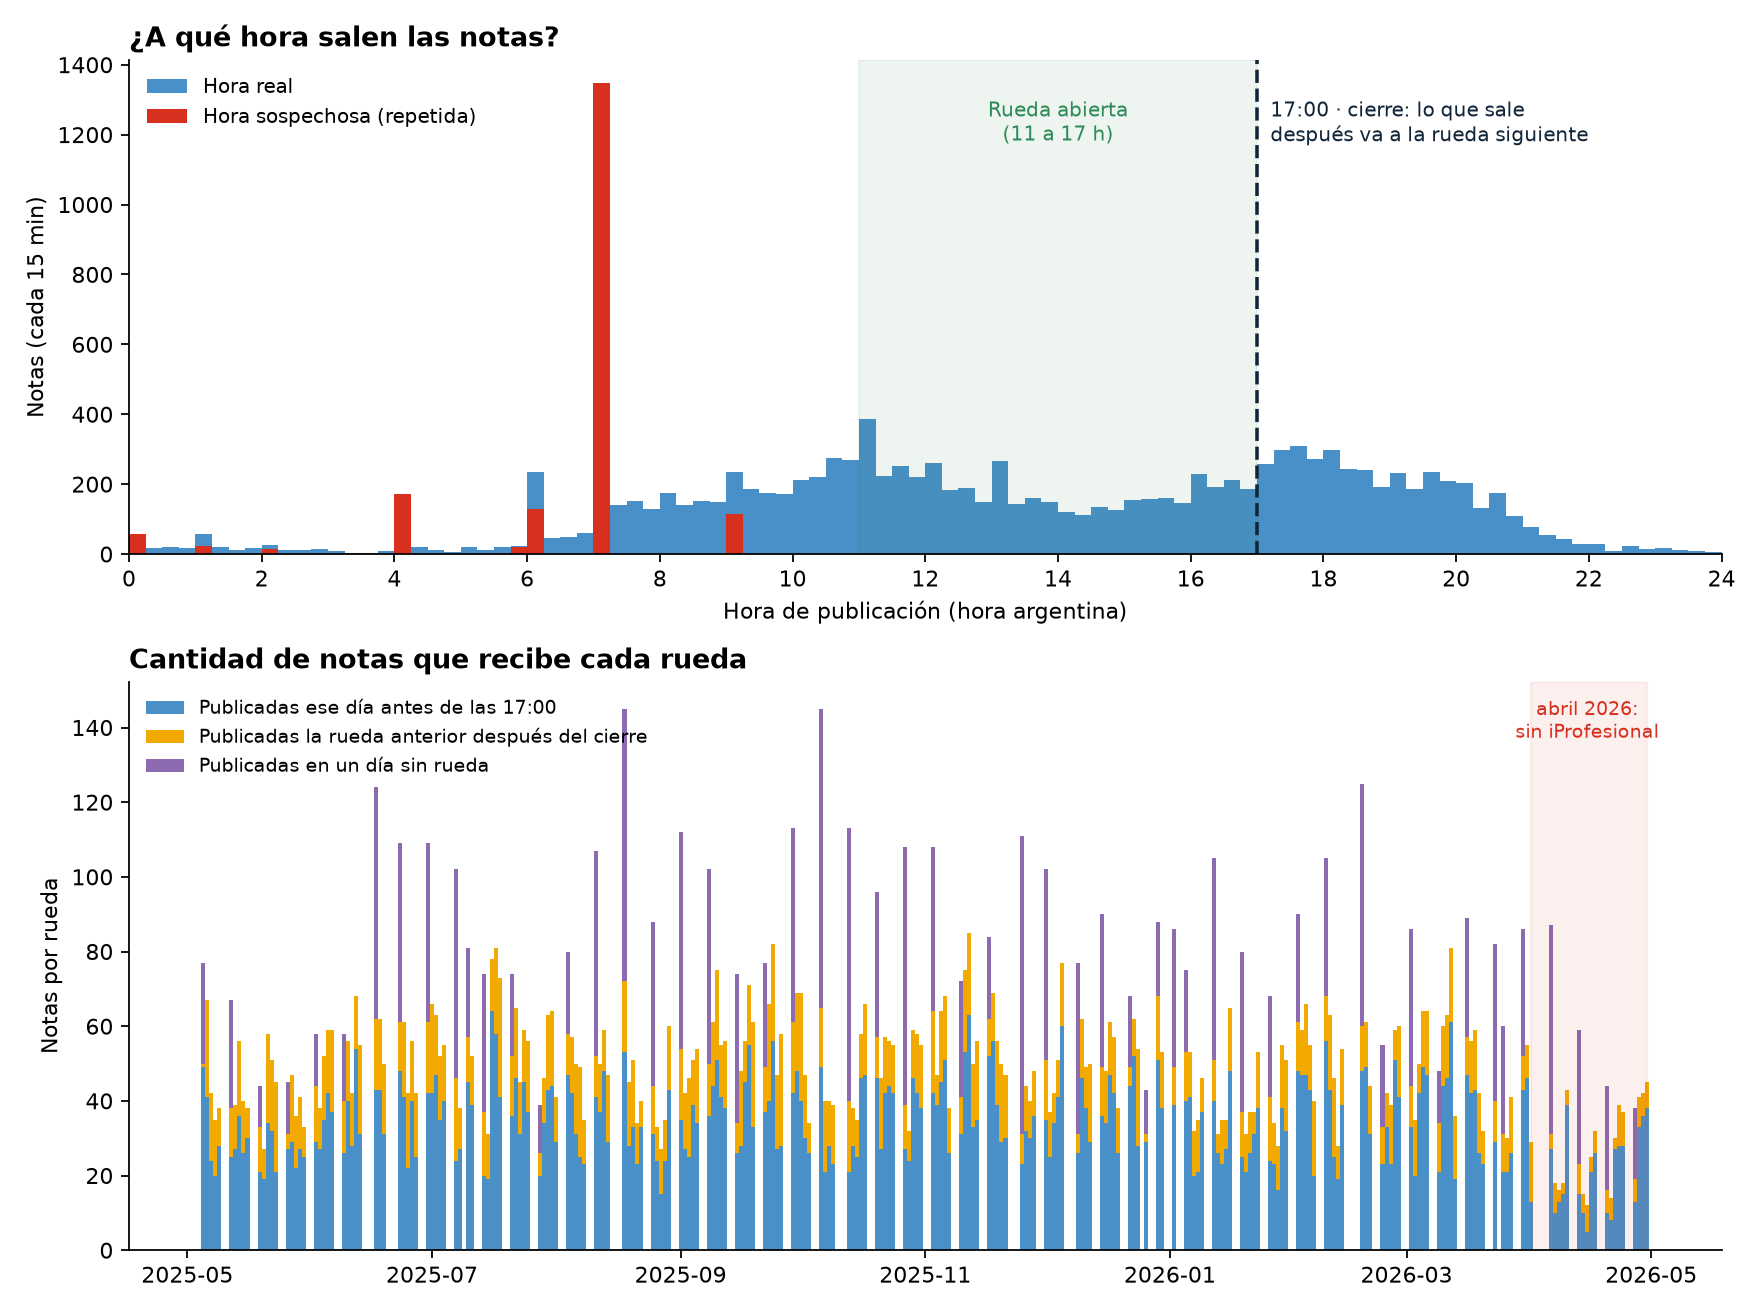
\includegraphics[width=0.76\linewidth]{regla_17.png}
\caption{Arriba: hora de publicación de las notas, con la rueda sombreada y el cierre de las
17:00; en rojo, horas repetidas que no pueden ser reales. Abajo: notas que recibe cada rueda, según
de dónde vienen. Fuente: elaboración propia (\carpeta{3_preparacion_de_los_datos/regla_17}).}
\label{fig:regla17}
\end{figure}

\textbf{Horas sospechosas.} El \dato{regla17.pct_hora_sospechosa}\% de las notas
(\dato{regla17.notas_hora_sospechosa}) tiene una hora que se repite demasiado dentro de su portal,
como las 07:00 de Clarín o las 00:00 de Ámbito: no es la hora real sino una hora por defecto del
sitio. Para esas notas la regla puede equivocarse de rueda; queda como limitación
(sección~\ref{sec:limites}). El paso pasó \dato{regla17.controles_ok} controles automáticos: por
ejemplo, ninguna nota va a una rueda anterior a su publicación.

% ---------------------------------------------------------------------
\section{El etiquetado con Gemma}
\label{sec:etiquetado}

Para entrenar un modelo de sentimiento hacen falta oraciones con su sentimiento ya marcado, y no
existía un conjunto público de prensa económica argentina. Se usó un modelo de lenguaje como
etiquetador, una práctica que puede igualar a anotadores contratados \citep{gilardi2023chatgpt} y
que también se evaluó en textos financieros \citep{aguda2024llmannot}. El etiquetador fue Gemma
\citep{gemma2026gemma4}, en su versión \texttt{gemma4:26b}, ejecutado en una computadora propia
con Ollama y con temperatura 0,1, para que respondiera siempre de la misma manera.

\textbf{El proceso, paso a paso.}
\begin{enumerate}[label=\arabic*.]
  \item \textbf{Selección.} Se tomó una noticia de cada una de las \dato{corpus.fuentes} fuentes por
        tanda, hasta \dato{gemma.noticias} noticias (entre \dato{gemma.noticias_fuente_min} y
        \dato{gemma.noticias_fuente_max} por fuente), para que ningún portal domine.
  \item \textbf{Contexto.} Gemma leyó el título, la bajada y los primeros 3.000 caracteres de la
        noticia, y escribió un análisis de contexto: tema central, encuadre, actores y sentimiento general.
  \item \textbf{Etiqueta por oración.} Con ese contexto como referencia, Gemma etiquetó cada oración
        de al menos 30 caracteres como positiva (POS), negativa (NEG), neutra (NEU) o mixta
        (MIXTO), con la instrucción de que el sentimiento surgiera de lo que la oración expresa por
        sí misma. Para cada oración devolvió la etiqueta, su confianza y una \textbf{razón} escrita.
  \item \textbf{Limpieza.} De las \dato{gemma.oraciones} oraciones etiquetadas se descartaron
        \dato{gemma.eliminadas}: textos repetidos, oraciones procesadas dos veces y restos del
        \textit{scraping} («PUBLICIDAD PUBLICIDAD PUBLICIDAD»). Quedaron \dato{gemma.limpias}.
\end{enumerate}

Antes de la limpieza, el \dato{gemma.pct_NEU}\% de las oraciones era neutra, el
\dato{gemma.pct_POS}\% positiva, el \dato{gemma.pct_NEG}\% negativa y el \dato{gemma.pct_MIXTO}\%
mixta. La tabla~\ref{tab:ejemplos} muestra ejemplos elegidos al azar (con semilla fija) entre
oraciones de noticias que FinBETO no vio al entrenar, con la razón que dio Gemma y lo que predijo
FinBETO (sección~\ref{sec:finbeto}).

{\footnotesize
\begin{longtable}{@{}L{1.5cm}L{4.8cm}L{1.3cm}L{1.5cm}L{4.3cm}@{}}
\toprule
\textbf{Caso} & \textbf{Oración} & \textbf{Gemma} & \textbf{FinBETO} & \textbf{Razón de Gemma} \\
\midrule
\endhead
\tabla{ejemplos}
\bottomrule
\caption{Ejemplos del etiquetado. Fuente: elaboración propia
(\carpeta{3_preparacion_de_los_datos/sentimiento_finbeto/salidas/ejemplos_etiquetado.csv}).}
\label{tab:ejemplos}
\end{longtable}
}

\textbf{Sin revisión humana.} Las etiquetas no se compararon con una muestra etiquetada por
personas. El F1 de FinBETO mide, entonces, su acuerdo con Gemma, no con un criterio humano; es una
limitación del trabajo (sección~\ref{sec:limites}).

% ---------------------------------------------------------------------
\section{De cuatro clases a tres}
\label{sec:tresclases}

La primera versión de FinBETO clasificaba en cuatro clases, con MIXTO para las oraciones que
combinan señales de los dos signos («no brinda financiación directa, pero hay bancos dispuestos a
otorgar créditos»). En esta versión, \textbf{las oraciones MIXTO pasaron a NEU}, sin volver a
etiquetar. Las razones son tres:

\begin{itemize}
  \item \textbf{No se usaba la diferencia.} El sentimiento neto de una nota
        (sección~\ref{sec:sentimiento}) es el porcentaje de oraciones positivas menos el de
        negativas: las mixtas ya aportaban 0, igual que las neutras. No había forma de justificar
        dos clases que se tratan igual.
  \item \textbf{Escala ordenada.} Con POS, NEU y NEG el sentimiento queda en una escala con orden
        ($+1$, $0$, $-1$). MIXTO no tenía lugar en esa escala: era una clase nominal.
  \item \textbf{Comparación justa.} El modelo de referencia clasifica en esas mismas tres clases.
\end{itemize}

Para que lo único que cambie sea la etiqueta, se usaron \textbf{exactamente las mismas oraciones}
que en la versión anterior, con el mismo sorteo, y recién después se reemplazó MIXTO por NEU
(\dato{fbdata.mixto_pasadas_a_neu} oraciones). Se pierde el matiz de «buena y mala noticia a la
vez», que queda para trabajos futuros.

% ---------------------------------------------------------------------
\section{FinBETO}
\label{sec:finbeto}

BERT \citep{devlin2019bert} es un modelo de lenguaje preentrenado con la tarea de adivinar palabras
ocultas en un texto. BETO es su versión en español \citep{canete2020beto}. Para clasificar
sentimiento se le agrega una capa de salida y se lo ajusta con oraciones etiquetadas
(\textit{fine-tuning}), como hizo FinBERT en inglés \citep{araci2019finbert}. Antes del ajuste
conviene seguir el preentrenamiento con texto del propio dominio \citep{gururangan2020dapt}.
FinBETO es el resultado de los dos pasos sobre la prensa económica argentina.

\textbf{Preentrenamiento continuado.} Se hizo en la versión anterior y no cambió: la tarea de
adivinar el 15\% de las palabras, ocultas al azar, sobre el texto de 14.667 notas, durante 3
épocas. Ante la frase «La [MASK] llegó al 3\% mensual según el INDEC», el modelo propone
«inflación» con probabilidad 0,81: ya habla el idioma de la prensa económica argentina.

\textbf{Ajuste fino.} Las oraciones se dividieron \textbf{por noticia}: todas las oraciones de una
nota van al mismo conjunto, de modo que la prueba mide al modelo sobre noticias que nunca vio
(tabla~\ref{tab:division}). Si se dividiera por oración, el modelo vería al entrenar otras
oraciones de la misma nota y el resultado saldría inflado \citep{kapoor2023leakage}. El sorteo se
hizo por portal y con semilla fija. Para que la clase neutra no dominara, se tomó un tope por clase,
y los errores en las clases menos frecuentes se penalizaron algo más\footnote{La pérdida se ponderó
por la raíz cuadrada de la frecuencia inversa de cada clase.}. Se entrenó 5 épocas, con lotes de
32, tasa de aprendizaje $2\cdot10^{-5}$ y selección de la mejor época por F1 macro en validación,
con \dato{fb.semillas} semillas distintas, porque la prueba es chica.

\begin{table}[H]
\centering\small
\begin{tabular}{@{}lrrrrr@{}}
\toprule
\textbf{Conjunto} & \textbf{Noticias} & \textbf{Oraciones} & \textbf{POS} & \textbf{NEG} & \textbf{NEU} \\
\midrule
\tabla{division_finbeto}
\bottomrule
\end{tabular}
\caption{División de las oraciones etiquetadas para el ajuste fino, por noticia. NEU incluye las
oraciones que eran MIXTO. Fuente: elaboración propia
(\carpeta{3_preparacion_de_los_datos/sentimiento_finbeto}).}
\label{tab:division}
\end{table}

\textbf{Evaluación.} En las \dato{fbcmp.completo.n} oraciones de prueba, FinBETO obtiene un
\textbf{F1 macro de \dato{fb.f1_macro_media@3}} ($\pm$ \dato{fb.f1_macro_desvio@3} entre
semillas). El modelo de referencia, \carpeta{finiteautomata/beto-sentiment-analysis}
\citep{perez2021pysentimiento}, es un BETO ajustado con tuits en las mismas tres clases y obtiene
\textbf{\dato{fbcmp.completo.referencia_f1_macro@3}}: FinBETO lo supera por
\textbf{\dato{fbcmp.completo.ventaja_puntos} puntos} (tabla~\ref{tab:finbeto}). El de referencia
clasifica como neutras \dato{fbcmp.completo.referencia_dice_neutro} de las
\dato{fbcmp.completo.n} oraciones: no entiende el lenguaje económico. Esta es la primera parte del
criterio de aceptación de H1.

\begin{table}[H]
\centering\footnotesize
\begin{tabular}{@{}lcc@{}}
\toprule
\textbf{Medida en la prueba (noticias no vistas)} & \textbf{FinBETO} & \textbf{Referencia} \\
\midrule
\tabla{finbeto}
\bottomrule
\end{tabular}
\caption{FinBETO contra el modelo de referencia. FinBETO: media de \dato{fb.semillas} semillas.
\textsuperscript{a}~Modelo final (semilla 42); en la versión anterior, con cuatro clases, era 0,724
contra 0,546. Fuente: elaboración propia (\carpeta{3_preparacion_de_los_datos/sentimiento_finbeto}).}
\label{tab:finbeto}
\end{table}

La matriz de confusión del modelo final (tabla~\ref{tab:matriz}) muestra dónde se equivoca: casi
nunca confunde una oración positiva con una negativa; los errores están entre una clase con signo y
la neutra. De las \dato{fbsplit.test_exmixto} oraciones de prueba que eran MIXTO, clasificó
\dato{fb.exmixto.NEU} como neutras, \dato{fb.exmixto.NEG} como negativas y \dato{fb.exmixto.POS}
como positivas.

\begin{table}[H]
\centering\small
\begin{tabular}{@{}lcccr@{}}
\toprule
 & \multicolumn{3}{c}{\textbf{Predicción de FinBETO}} & \\
\cmidrule(lr){2-4}
\textbf{Etiqueta de Gemma} & \textbf{POS} & \textbf{NEG} & \textbf{NEU} & \textbf{Total} \\
\midrule
\tabla{matriz_finbeto}
\bottomrule
\end{tabular}
\caption{Matriz de confusión de FinBETO en la prueba (modelo final). La diagonal son los aciertos.
Fuente: elaboración propia (\carpeta{3_preparacion_de_los_datos/sentimiento_finbeto}).}
\label{tab:matriz}
\end{table}

% ---------------------------------------------------------------------
\section{El sentimiento de cada nota y de cada rueda}
\label{sec:sentimiento}

FinBETO clasificó las \dato{fbclas.oraciones_clasificadas} oraciones del corpus, con la misma
división en oraciones de la versión anterior, para que el cruce con las entidades
(sección~\ref{sec:propio}) siga valiendo. Sin contar \dato{fbnota.oraciones_relleno_excluidas}
oraciones de relleno, cada nota tiene su \textbf{sentimiento neto}:
\begin{equation}
S_j = 100\cdot\frac{n^{\text{POS}}_j - n^{\text{NEG}}_j}{n_j},
\end{equation}
donde $n_j$ es la cantidad de oraciones de la nota $j$ y $n^{\text{POS}}_j$ y $n^{\text{NEG}}_j$,
las positivas y las negativas. Va de $-100$ (todas negativas) a $+100$ (todas positivas). El
\textbf{sentimiento de la rueda} $\bar S_t$ es el promedio del de sus notas, cada nota con el mismo
peso. El \dato{fbacuerdo.acuerdo_pct}\% de las oraciones tiene la misma etiqueta que con el modelo
de cuatro clases (contando MIXTO como NEU), y la serie por rueda correlaciona
\dato{rueda.correlacion_con_5.0_sent_neto} con la anterior. El modelo nuevo es algo más negativo:
el promedio del período bajó de $+3{,}9$ a \dato{rueda.sent_neto_media@1} puntos.

\textbf{Sentimiento inesperado.}
\label{sec:inesperado}
Lo que interesa no es si las noticias son positivas en general, sino si una rueda es más positiva
o más negativa \textit{que lo habitual}. El \textbf{sentimiento inesperado} compara cada rueda con
el promedio de las 20 anteriores:
\begin{equation}
I_t = \bar S_t - \frac{1}{20}\sum_{k=1}^{20} \bar S_{t-k}.
\end{equation}
Vale 0 en una rueda habitual, y es el mismo valor para todas las acciones en esa rueda. Usa solo
ruedas anteriores, así que se conoce al cierre de $t$; las primeras 20 ruedas quedan sin valor. Su
desvío es de \dato{rueda.inesperado_desvio@1} puntos (figura~\ref{fig:sentimiento}).

\textbf{Por qué 20 ruedas.} Veinte ruedas son un mes de mercado: es el horizonte del VIX de
Chicago, que mide la volatilidad de los próximos 30 días corridos, unas 21 ruedas
\citep{cboe_vix}, y el del componente mensual del modelo de volatilidad de \citet{corsi2009}, de
22 días. Es también la ventana del VIX argentino y del volumen anormal, de modo que las tres
variables se comparan con el mismo «mes habitual». No se eligió con los datos: siguiendo a
\citet{tetlock2007}, que compara el volumen con su promedio móvil y verifica otras ventanas, el
anexo de robustez repite todo con 10 y con 60 ruedas (sección~\ref{sec:robustez}). Con 60, además,
se pierde el primer cuarto de la muestra.

\begin{figure}[H]
\centering
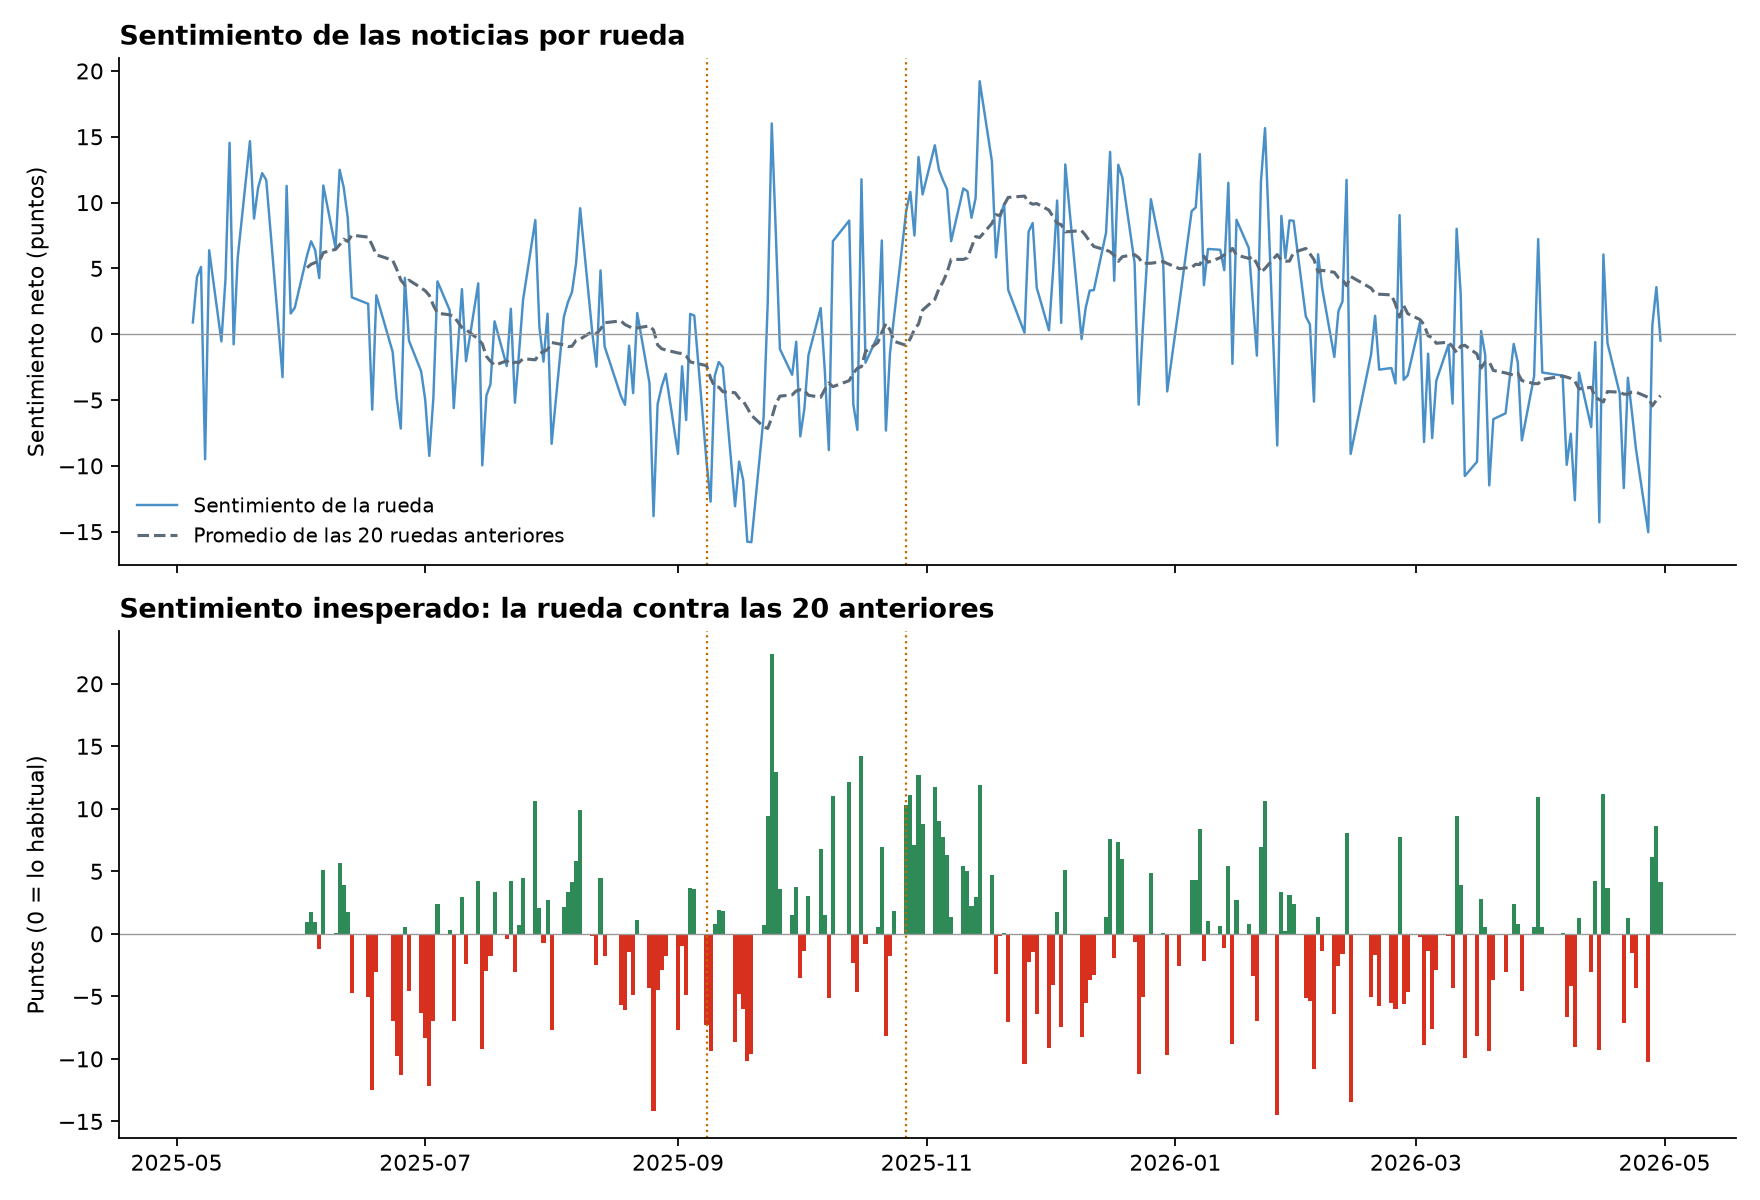
\includegraphics[width=0.78\linewidth]{sentimiento_por_rueda.png}
\caption{Arriba: sentimiento de cada rueda y promedio de las 20 ruedas anteriores. Abajo:
sentimiento inesperado (verde, más positivo que lo habitual; rojo, más negativo). Las líneas
punteadas son los días electorales. Fuente: elaboración propia
(\carpeta{3_preparacion_de_los_datos/sentimiento_por_rueda}).}
\label{fig:sentimiento}
\end{figure}

% ---------------------------------------------------------------------
\section{El sentimiento propio de cada empresa}
\label{sec:propio}

El sentimiento inesperado mide el clima de las noticias en general. Para saber de qué empresa habla
cada oración se usó el reconocimiento de entidades nombradas (NER), que identifica nombres de
organizaciones en un texto \citep{tjongkimsang2002conll}. Se combinó el modelo
\texttt{es\_core\_news\_lg} de spaCy \citep{honnibal2020spacy} con un diccionario de las
\dato{mercado.acciones} empresas del panel, donde cada alias se resuelve a su ticker: «Banco
Galicia», «Grupo Financiero Galicia» y «GGAL» cuentan como una sola empresa. Cada mención se unió
con el sentimiento de su oración, exigiendo que el texto coincida: se unieron el
\dato{empresa.cobertura_cruce_pct}\% de las oraciones con entidades.

El sentimiento de la empresa $i$ en la rueda $t$ es el de las oraciones que la mencionan,
$S_{i,t} = 100\cdot(n^{\text{POS}}_{i,t} - n^{\text{NEG}}_{i,t})/n_{i,t}$. Como la mediana es de
\dato{empresa.mediana_oraciones_por_rueda_empresa} oraciones por rueda, y en el
\dato{empresa.pct_ruedas_empresa_una_oracion}\% de las ruedas hay una sola, ese valor sale muchas
veces todo o nada. Por eso se lo \textit{encoge} hacia el sentimiento del mercado según la cantidad
de oraciones \citep{efron1975}. El \textbf{sentimiento propio} es:
\begin{equation}
P_{i,t} =
\begin{cases}
\dfrac{n_{i,t}}{n_{i,t} + K}\,\bigl(S_{i,t} - \bar S_t\bigr) & \text{si alguna oración de la rueda menciona a la empresa,}\\[8pt]
0 & \text{si no.}
\end{cases}
\end{equation}
Mide cuánto mejor o peor se habló de la empresa que del mercado ese mismo día. $K$ sale de los
datos: es la varianza del sentimiento de una oración suelta dividida por la varianza real del
sentimiento relativo entre días. Para que el período de prueba no influya en ninguna variable, se
estimó \textbf{solo con las ruedas de entrenamiento}: $K = \dato{dataset.k_peso_entrenamiento}$
(con todas las ruedas daba \dato{dataset.k_peso_todas_las_ruedas}, y las dos versiones
correlacionan \dato{dataset.correlacion_sentimiento_propio_k_entrenamiento_vs_k_todas}). Con una
oración el peso es \dato{dataset.peso_con_1_oraciones@2}, con diez \dato{dataset.peso_con_10_oraciones@2}
y con treinta \dato{dataset.peso_con_30_oraciones@2}.

\textbf{Las \dato{dataset.empresas} empresas.} Para medir el sentimiento propio, una empresa tiene
que tener noticias en buena parte de las ruedas. Con un corte de 90 de las \dato{dataset.ruedas}
ruedas quedan \dato{dataset.empresas} (figura~\ref{fig:cobertura}); el resto tiene pocas o
ninguna mención. Aun en esas \dato{dataset.empresas}, solo el \dato{dataset.pct_filas_con_noticia}\%
de las combinaciones de empresa y rueda tiene noticias. Por eso el modelo recibe, además, la
variable \var{hubo\_noticia}, que distingue «se habló de la empresa igual que del mercado»
($P_{i,t}=0$ con noticias) de «no se habló» ($P_{i,t}=0$ sin noticias).

\begin{figure}[H]
\centering
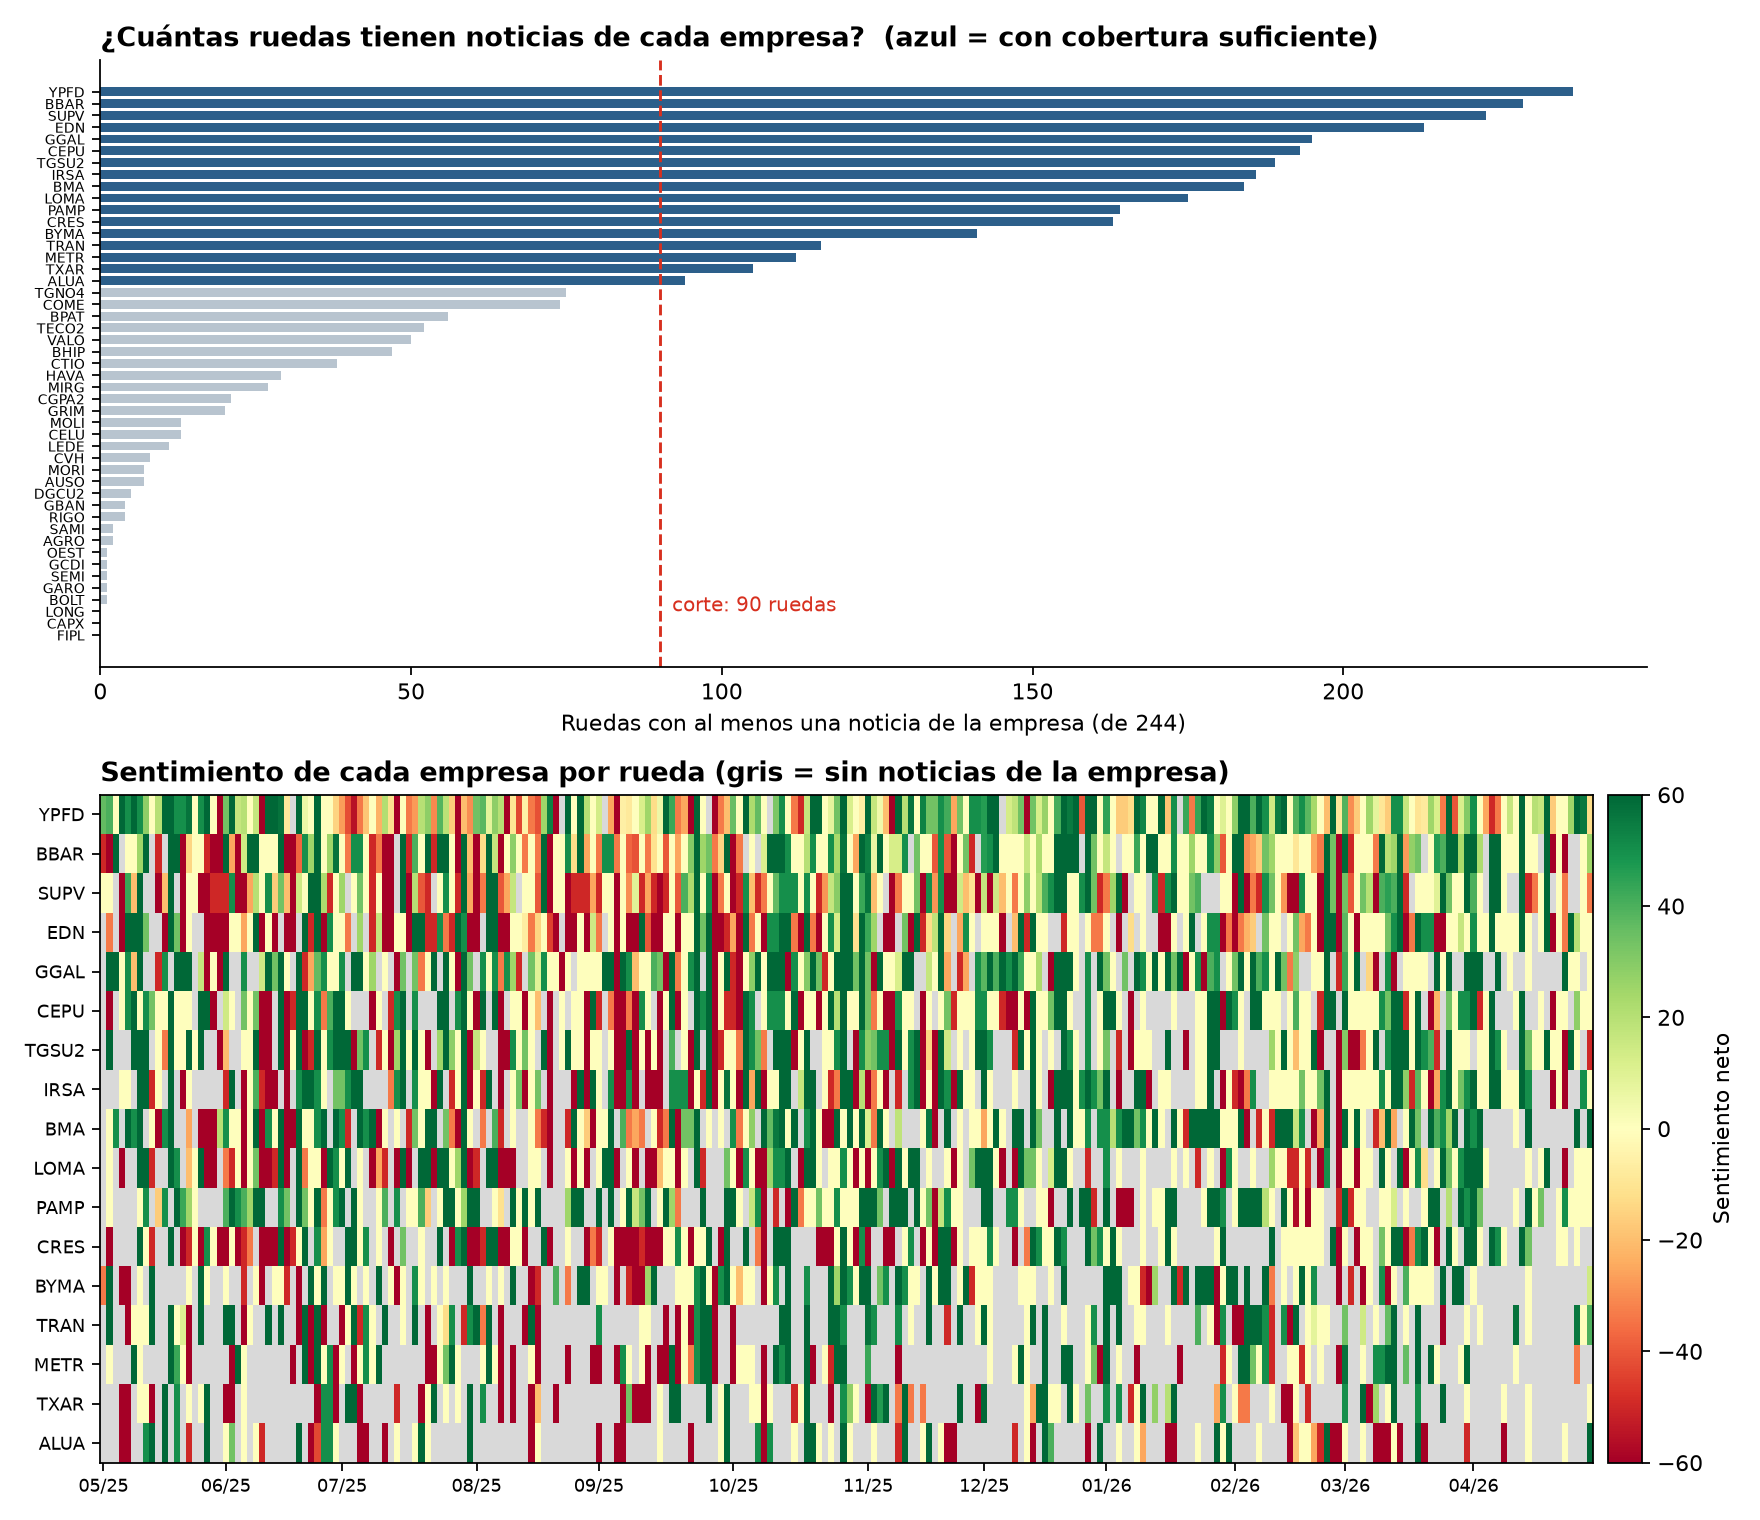
\includegraphics[width=0.6\linewidth]{cobertura_empresas.png}
\caption{Arriba: ruedas con al menos una noticia de cada empresa (en azul, las
\dato{dataset.empresas} con cobertura suficiente). Abajo: sentimiento de esas empresas en cada
rueda; en gris, ruedas sin noticias de la empresa. Fuente: elaboración propia
(\carpeta{3_preparacion_de_los_datos/sentimiento_por_empresa}).}
\label{fig:cobertura}
\end{figure}

% ---------------------------------------------------------------------
\section{Las variables del mercado}
\label{sec:vix}

\textbf{Retorno.} Es la variación porcentual del precio de cierre de una rueda a la siguiente:
\begin{equation}
r_{i,t} = \frac{P_{i,t} - P_{i,t-1}}{P_{i,t-1}}.
\end{equation}
Se usa la variación y no el precio porque se puede comparar entre acciones: \$100 en una acción y
\$100 en otra no significan lo mismo, un $+3\%$ sí.

\textbf{Volumen anormal.} El volumen es la cantidad de acciones operadas en la rueda. Como una
empresa grande opera millones y una chica muy pocas, se lo compara con el de la propia acción en
las 20 ruedas anteriores, en logaritmos:
\begin{equation}
V_{i,t} = \ln(1 + v_{i,t}) - \frac{1}{20}\sum_{k=1}^{20}\ln(1 + v_{i,t-k}).
\end{equation}
Vale 0 en una rueda habitual; $+0{,}69$ es el doble de lo habitual y $-0{,}69$, la mitad.

\textbf{VIX argentino.} Mide cuánta tensión hay en el mercado. Es la \textit{volatilidad
realizada} del S\&P~Merval: el desvío estándar de sus retornos diarios en las últimas 20 ruedas,
anualizado \citep{sakowski2023}:
\begin{equation}
\sigma_t = \sqrt{252}\cdot\operatorname{desv}\left(r_{t-19},\dots,r_t\right)\cdot 100,
\end{equation}
donde $r_t$ es el retorno del índice y $\sqrt{252}$ lleva el desvío diario a una escala anual
comparable con la de cualquier otro índice. Un VIX de 40\% quiere decir que, al ritmo del último
mes, el índice se movería en un año alrededor de un 40\% hacia arriba o hacia abajo. En la ventana,
el promedio fue de \dato{vix.vix_media}\%, con un mínimo de \dato{vix.vix_min}\%
(\dato{vix.vix_min_fecha}) y un máximo de \dato{vix.vix_max}\% (\dato{vix.vix_max_fecha}), la
última rueda en que la suba del 27/10/2025, posterior a las elecciones legislativas, seguía dentro
de la ventana de 20 ruedas.

\textbf{Escala.} Para leer el VIX se lo dividió en tres niveles, por terciles de las
\dato{vix.ruedas_ventana} ruedas de la ventana (tabla~\ref{tab:escala-vix}): \textit{bajo} es el
tercio de ruedas con menor volatilidad, \textit{alto} el tercio con mayor volatilidad. La escala
sale de los datos y no depende de ningún modelo. El VIX de Estados Unidos se suele leer con
umbrales de 20 y 30, pero no sirven para Argentina, donde el promedio supera el 40\%.

\begin{table}[H]
\centering\small
\begin{tabular}{@{}llrrr@{}}
\toprule
\textbf{Nivel} & \textbf{VIX argentino} & \textbf{Ruedas} & \textbf{VIX promedio} & \textbf{Ruedas del test} \\
\midrule
\tabla{vix_escala}
\bottomrule
\end{tabular}
\caption{Escala del VIX argentino por terciles de la ventana (\dato{vix.ruedas_ventana} ruedas). La
última columna cuenta las ruedas del período de prueba del modelo (capítulo~\ref{cap:modelado}).
Fuente: elaboración propia (\carpeta{3_preparacion_de_los_datos/vix_argentino}).}
\label{tab:escala-vix}
\end{table}

\begin{figure}[H]
\centering
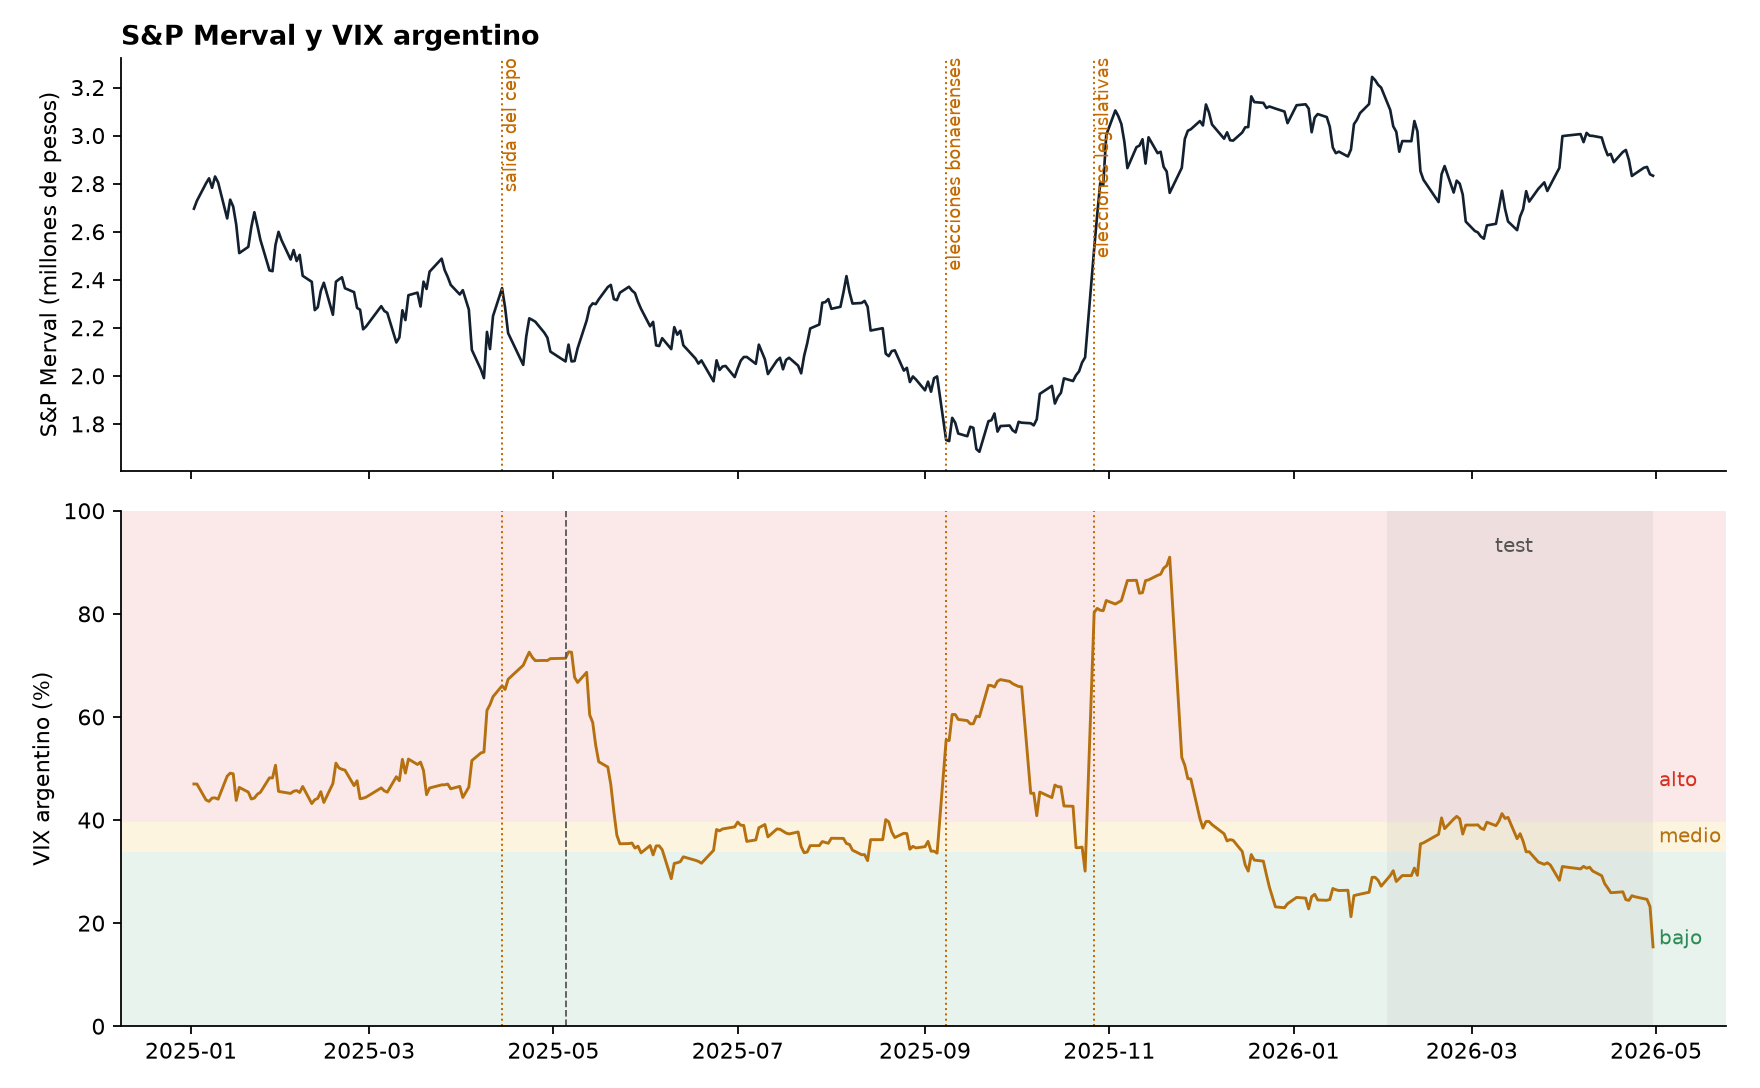
\includegraphics[width=0.86\linewidth]{vix_arg.png}
\caption{S\&P~Merval en pesos (arriba) y VIX argentino (abajo), con los tres niveles de la escala
sombreados. Las líneas punteadas marcan la salida del cepo (14/04/2025) y las elecciones
bonaerenses (07/09/2025) y legislativas (26/10/2025); la línea discontinua, el comienzo de la
ventana, y el sombreado gris, el período de prueba. Fuente: elaboración propia con datos de Yahoo
Finance (\carpeta{3_preparacion_de_los_datos/vix_argentino}).}
\label{fig:vix}
\end{figure}

Una regla de lectura: como el VIX es un desvío de 20 ruedas, un único día extremo queda dentro del
cálculo durante exactamente 20 ruedas. El índice salta el día del shock y cae de golpe 20 ruedas
después, aunque ese día el mercado no haga nada especial \citep{papaioannou2014}. La misma regla
vale para el sentimiento inesperado y el volumen anormal.

% ---------------------------------------------------------------------
\section{El dataset unificado}
\label{sec:dataset}

Todo se juntó en una tabla con una fila por acción y por rueda: \dato{dataset.empresas} empresas
$\times$ \dato{dataset.ruedas} ruedas $=$ \textbf{\dato{dataset.filas_panel} filas}
(figura~\ref{fig:panorama}). Para la dirección inversa, en la que se predice el sentimiento del
mercado, se armó además una tabla con una fila por rueda. El retorno, el volumen anormal y el VIX
son idénticos a los de la versión anterior, y la preparación pasó todos sus controles
automáticos: por ejemplo, ninguna variable de la rueda $t$ usa información posterior al cierre de
$t$.

\begin{figure}[H]
\centering
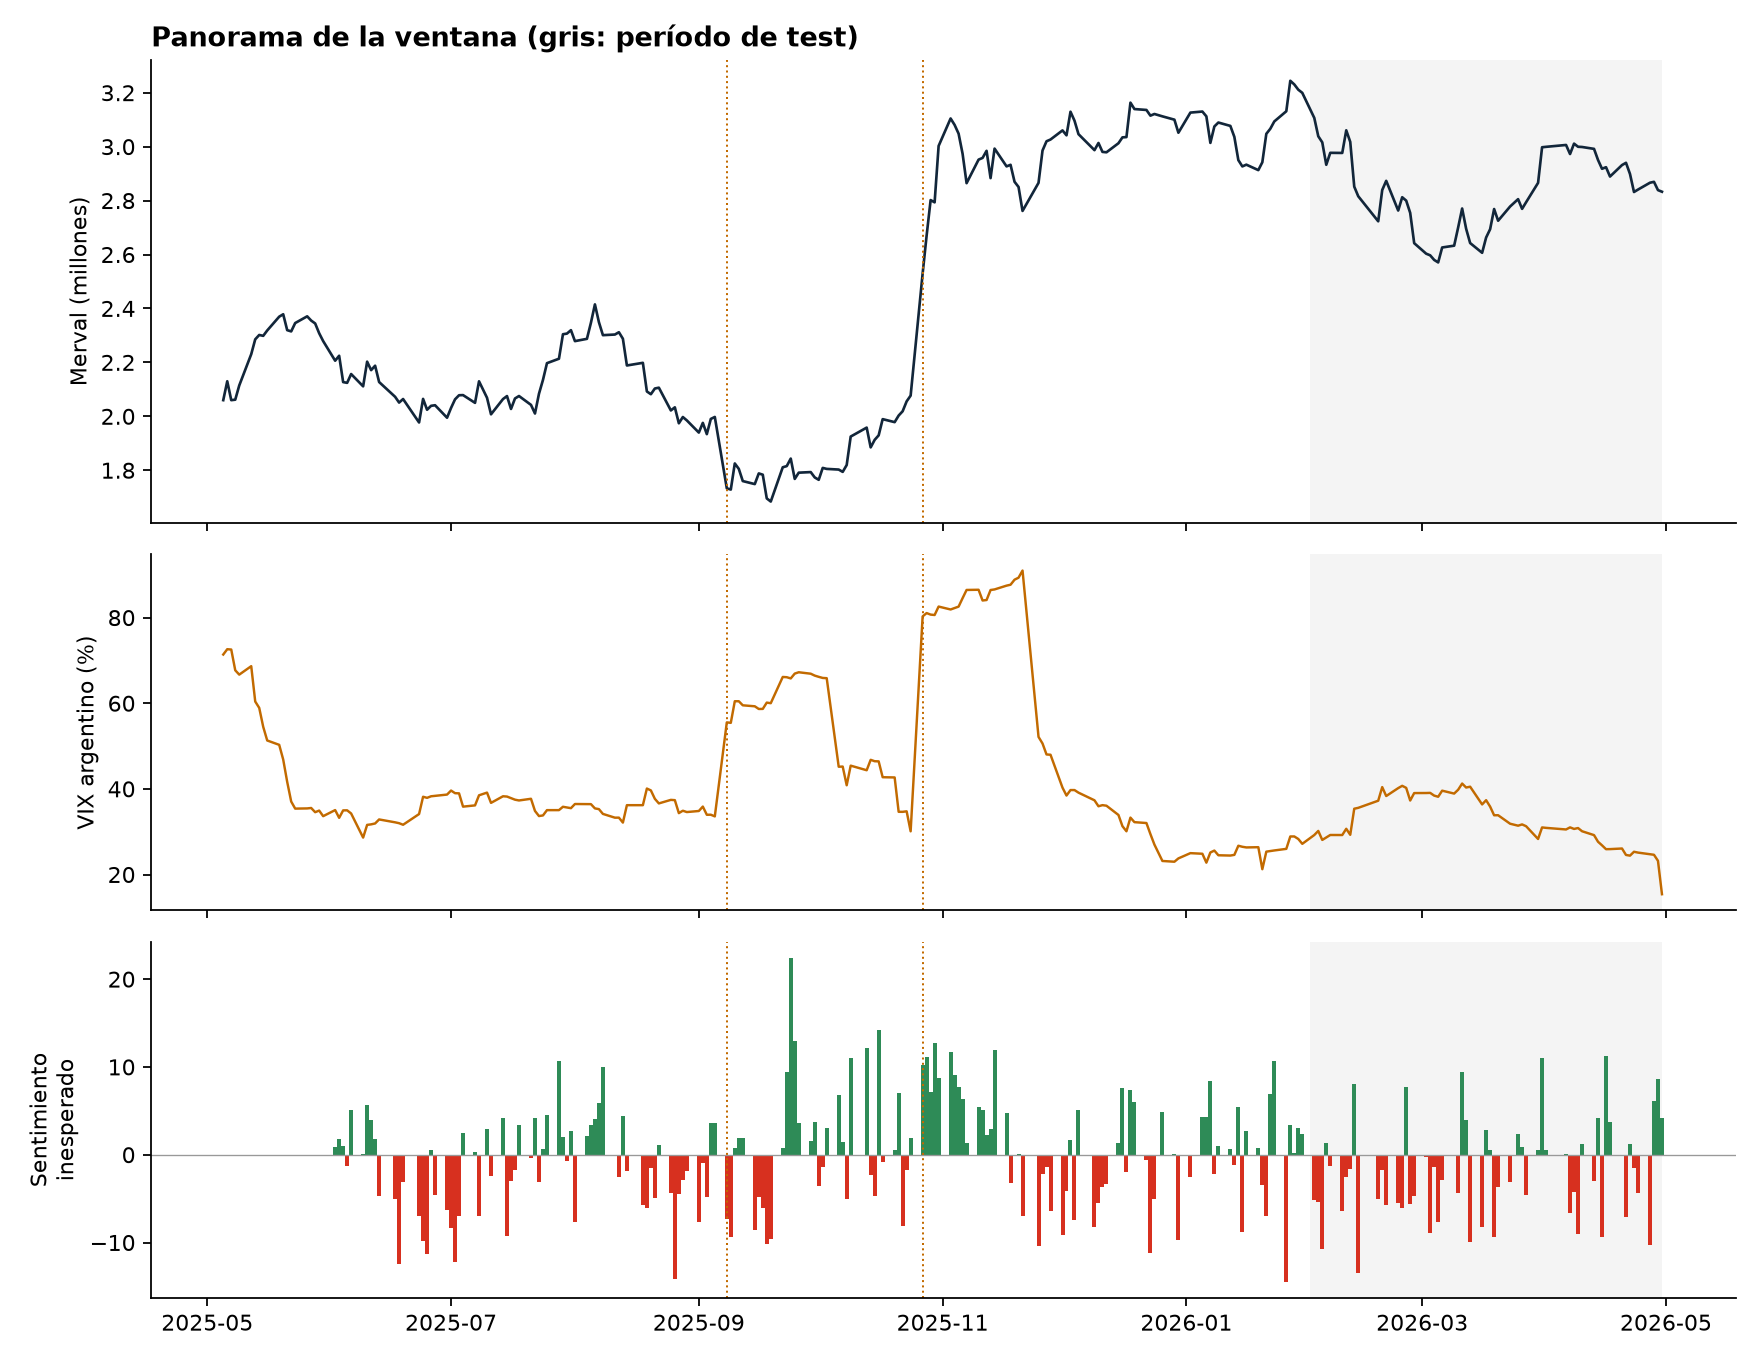
\includegraphics[width=0.78\linewidth]{panorama.png}
\caption{La ventana de estudio: S\&P~Merval, VIX argentino y sentimiento inesperado. En gris, el
período de prueba del modelo. Fuente: elaboración propia
(\carpeta{3_preparacion_de_los_datos/dataset_unificado}).}
\label{fig:panorama}
\end{figure}
